\documentclass[11pt]{beamer}
\graphicspath{{img/}{./}}
\usepackage[french]{babel}
\usepackage{graphicx}
\usepackage{ulem} %Pour biffer du texte \sout{texte barré}
\usepackage{xcolor} 
\usepackage{tabularx}
\usepackage{parallel}
%\usepackage[babelshorthands]{polyglossia}
\usepackage{ragged2e} 


%Allignemebnt droite/gauche
\usepackage{polyglossia}
%\usepackage[babelshorthands]{polyglossia} %[babelshorthands] permet d'avoir les guillemets allemands avec le code "`toto"' et les guillemets français avec le code "<tata">


\usepackage{multirow} 
\setmainlanguage{english}
\usepackage[autostyle]{csquotes}
\MakeOuterQuote{"}
\DeclareQuoteStyle{english}%
    {\textquotedblleft}
    [\textquotedblleft]
    {\textquotedblright}
        [0.05em]
    {\textquoteleft}
    [\textquoteleft]
    {\textquoteright}
% \DeclareQuoteStyle[quotes]{french}
%   {\mkfrenchopenquote{«}}
%   {\mkfrenchclosequote{\nobreakspace»}}
%   {\textquotedblleft}
%   {\textquotedblright}
% \DeclareQuoteStyle[quotes*]{french}
%   {\mkfrenchopenquote{«}}
%   {\mkfrenchclosequote{\nobreakspace»}}
%   {\mkfrenchopenquote{\textquotedblleft}}
%   {\mkfrenchclosequote{\textquotedblright}}
% \DeclareQuoteStyle[guillemets]{french}
%   [\initfrenchquotes]
%   {\mkfrenchopenquote{«}}
%   [\mkfrenchopenquote{«}]
%   {\mkfrenchclosequote{\nobreakspace»}}
%   {\mkfrenchopenquote{«}}
%   [\mkfrenchopenquote{«}]
%   {\mkfrenchclosequote{\nobreakspace»}}
% \DeclareQuoteStyle[guillemets*]{french}
%   [\initfrenchquotes]
%   {\mkfrenchopenquote{«}}
%   [\mkfrenchopenquote{\nobreakspace»}]
%   {\mkfrenchclosequote{\nobreakspace»}}
%   {\mkfrenchopenquote{«}}
%   [\mkfrenchopenquote{\nobreakspace»}]
%   {\mkfrenchclosequote{\nobreakspace»}}




\setotherlanguage{greek}
\newfontfamily\greekfont[Script=Greek]{Linux Libertine O}
\newfontfamily\greekfontsf[Script=Greek]{Linux Libertine O}
\setotherlanguage{hebrew}
\newfontfamily{\hebrewfont}[Script=Hebrew, Path=./fonts/]{SBL_Hbrw.ttf}
\newfontfamily{\hebrewfontsf}[Script=Hebrew]{Miriam CLM}
\newfontfamily{\hebrewfonttt}[Script=Hebrew]{Miriam Mono CLM}
\setotherlanguage{syriac}
\newfontfamily\syriacfont[Script=Syriac, Path=./fonts/]{EstrangeloEdessa.ttf}

\usepackage{booktabs} % Allows the use of \toprule, \midrule and \bottomrule for better rules in tables
%% Allow the use of tcolorbox
\usepackage[skins]{tcolorbox}
%\usetheme{default}
%\usetheme{AnnArbor}
%\usetheme{Antibes}
%\usetheme{Bergen}
%\usetheme{Berkeley}
%\usetheme{Berlin}
%\usetheme{Boadilla}
%\usetheme{CambridgeUS}
%\usetheme{Copenhagen}
%\usetheme{Darmstadt}
%\usetheme{Dresden}
%\usetheme{Frankfurt}
%\usetheme{Goettingen}
%\usetheme{Hannover}
%\usetheme{Ilmenau}
\usetheme{JuanLesPins}
%\usetheme{Luebeck}
%\usetheme{Madrid}
%\usetheme{Malmoe}
%\usetheme{Marburg}
%\usetheme{Montpellier}
%\usetheme{PaloAlto}
%\usetheme{Pittsburgh}
%\usetheme{Rochester}
%\usetheme{Singapore}
%\usetheme{Szeged}
%\usetheme{Warsaw}

%----------------------------------------------------------------------------------------
%	SELECT COLOR THEME
%----------------------------------------------------------------------------------------

% Beamer comes with a number of color themes that can be applied to any layout theme to change its colors. Uncomment each of these in turn to see how they change the colors of your selected layout theme.

%\usecolortheme{albatross}
%\usecolortheme{beaver}
%\usecolortheme{beetle}
%\usecolortheme{crane}
%\usecolortheme{dolphin}
%\usecolortheme{dove}
%\usecolortheme{fly}
%\usecolortheme{lily}
%\usecolortheme{monarca}
%\usecolortheme{seagull}
%\usecolortheme{seahorse}
%\usecolortheme{spruce}
%\usecolortheme{whale}
%\usecolortheme{wolverine}

%----------------------------------------------------------------------------------------
%	SELECT FONT THEME & FONTS
%----------------------------------------------------------------------------------------
\setmainfont{cochineal}
% Beamer comes with several font themes to easily change the fonts used in various parts of the presentation. Review the comments beside each one to decide if you would like to use it. Note that additional options can be specified for several of these font themes, consult the beamer documentation for more information.

%\usefonttheme{default} % Typeset using the default sans serif font
\usefonttheme{serif} % Typeset using the default serif font (make sure a sans font isn't being set as the default font if you use this option!)
%\usefonttheme{structurebold} % Typeset important structure text (titles, headlines, footlines, sidebar, etc) in bold
%\usefonttheme{structureitalicserif} % Typeset important structure text (titles, headlines, footlines, sidebar, etc) in italic serif
%\usefonttheme{structuresmallcapsserif} % Typeset important structure text (titles, headlines, footlines, sidebar, etc) in small caps serif

%------------------------------------------------

%\usepackage{mathptmx} % Use the Times font for serif text
%\usepackage{palatino} % Use the Palatino font for serif text


%\usepackage{helvet} % Use the Helvetica font for sans serif text
%\usepackage[default]{opensans} % Use the Open Sans font for sans serif text
%\usepackage[default]{FiraSans} % Use the Fira Sans font for sans serif text
%\usepackage[default]{lato} % Use the Lato font for sans serif text

%----------------------------------------------------------------------------------------
%	SELECT INNER THEME
%----------------------------------------------------------------------------------------

% Inner themes change the styling of internal slide elements, for example: bullet points, blocks, bibliography entries, title pages, theorems, etc. Uncomment each theme in turn to see what changes it makes to your presentation.

%\useinnertheme{default}
%\useinnertheme{circles}
\useinnertheme{rectangles}
%\useinnertheme{rounded}
%\useinnertheme{inmargin}

%----------------------------------------------------------------------------------------
%	SELECT OUTER THEME
%----------------------------------------------------------------------------------------

% Outer themes change the overall layout of slides, such as: header and footer lines, sidebars and slide titles. Uncomment each theme in turn to see what changes it makes to your presentation.

%\useoutertheme{default}
%\useoutertheme{infolines}
%\useoutertheme{miniframes}
%\useoutertheme{smoothbars}
%\useoutertheme{sidebar}
%\useoutertheme{split}
%\useoutertheme{shadow}
%\useoutertheme{tree}
%\useoutertheme{smoothtree}

%\setbeamertemplate{footline} % Uncomment this line to remove the footer line in all slides
%\setbeamertemplate{footline}[page number] % Uncomment this line to replace the footer line in all slides with a simple slide count

%\setbeamertemplate{navigation symbols}{} % Uncomment this line to remove the navigation symbols from the bottom of all slides
\usepackage[style=sbl]{biblatex}


\DeclareSourcemap{
  \maps[datatype=bibtex]{
    \map{
      \step[fieldset=doi, null]
      \step[fieldset=language, null]
      \step[fieldset=issn, null]{}
      \step[fieldset=url, null]{}
      \step[fieldset=isbn, null]{}
      \step[fieldset=eprint, null]{}
    }
  }
}

\addbibresource{references.bib}
%\defbibheading{bibempty}{}

%----------
% Define sectioning
\AtBeginSection[]{
  \begin{frame}
  \vfill
  \centering
  \begin{beamercolorbox}[sep=8pt,center,shadow=true,rounded=true]{title}
    \usebeamerfont{title}\insertsectionhead\par%
  \end{beamercolorbox}
  \vfill
  \end{frame}
}

%-----------

%----------------------------------------------------------------------------------------
%	PRESENTATION INFORMATION
%----------------------------------------------------------------------------------------


\title{Introduction à la critique textuelle}
\author[Frédérique Michèle Rey, Sophie Robert-Hayek]{Frédérique Michèle Rey \& Sophie Robert-Hayek}


\institute[UL]{Université de Lorraine } %\smallskip \textit{frederique.rey@univ-lorraine.fr / sophie.robert@univ-lorraine.fr}}

\date{}
\setbeamertemplate{footline}[frame number]

\usepackage[table]{xcolor}
\usepackage[dvipsnames]{xcolor}
\usepackage{forest}
\usepackage{tikz-qtree}
\usepackage[font=scriptsize]{caption}
\begin{document}
\title{Introduction à la critique textuelle}
\subtitle{Critique textuelle du Nouveau Testament}

\begin{frame}{}
    \titlepage
\end{frame}

\begin{frame}{Plan du cours}
\tableofcontents
\end{frame}

\section{Introduction}

\begin{frame}{La transmission des textes}
    \begin{block}{}
        Jusqu'à l'invention de l'imprimerie (XV\ieme{}), les textes en Europe ont circulé en \textbf{étant copié de manière successive par des scribes}.
    \end{block}
    Au fil des siècles:
    \begin{itemize}
        \item Des modifications \textbf{intentionnelles} et \textbf{non-intentionnelles} ont été introduites par les scribes;
        \item De nombreuses traductions ont été traduites.
    \end{itemize}
\end{frame}

\section{Définitions}




\begin{frame}{Définition et objectifs}

    Face à la multiplicité des textes:

    \begin{alertblock}{La critique textuelle}
        La critique textuelle est une science qui \textbf{étudie la rédaction} et les \textbf{circonstances de rédaction} des \textbf{textes anciens}.
    \end{alertblock}
    \pause

        La critique textuelle a plusieurs buts :
    \begin{itemize}

        \item Établir un texte \og d'origine \fg\ ;
        \pause
        \item Proposer des éditions critiques permettant une vue d'ensemble des variants textuels;
        \pause
        \item Comprendre la transmission des traditions textuelles et leurs milieux d'émergence.
    \end{itemize}
\end{frame}

\begin{frame}{Définition et objectif}
    \begin{alertblock}{}
\textbf{ATTENTION}: il ne faut pas confondre \textbf{critique textuelle} et \textbf{critique des sources}.
    \end{alertblock}
La critique des sources a pour objectif de \textbf{trouver des sources qui seraient sous-jacentes au texte néo-testamentaire}, par l'étude:
\begin{itemize}
    \item du style, du vocabulaire;
    \item des études comparatives avec d'autres \oe{}uvres;
    \item le contexte historique de rédaction.
\end{itemize}
\end{frame}
\begin{frame}{Définition et objectifs}
    Les difficultés principales résident :
    \begin{itemize}
        \item dans le fait que le texte d'origine (pour peu qu'il ait existé) n'est plus \textbf{disponible};
        \item L'histoire de la transmission des textes est \textbf{extrêmement compliquée}.
    \end{itemize}
    
\end{frame}


\begin{frame}{Définition et objectifs}

    \begin{alertblock}{}
La critique textuelle vise à \textbf{proposer un ensemble d'outils} permettant d'étudier \textbf{la transmission du texte}.
    \end{alertblock}

Ces méthodes ont pour résultat:
\begin{itemize}
    \item Des éditions éclectiques (avec ou sans apparat);
    \item Des éditions diplomatiques (avec ou sans apparat);
    \item Des \textit{stemma codicum};
    \item Des hypothèses quant à la genèse et l'évolution du texte néo-testamentaire.
\end{itemize}
\end{frame}

\begin{frame}{Définition et objectifs}
    \begin{alertblock}{}
Depuis l'ère moderne, \textbf{la critique textuelle du Nouveau Testament est très orientée vers l’éclectisme}.
    \end{alertblock}

La recherche moderne tente de s'en défaire, notamment par certains travaux sur \emph{le Codex de Bèze}.
\end{frame}

\begin{frame}{Définition et objectifs}
La critique textuelle concerne donc \textbf{l'ensemble des textes qui ont été écrits avant l'invention de l'imprimerie}, et n'est pas limitée à la Bible!\\

\begin{block}{}
    Le texte néo-testamentaire présente cependant qui le différencie des autres textes:
    \begin{itemize}
\item Il s'agit de l'une des \oe{}uvres littéraires les plus importantes de l'histoire occidentale;
\item Il s'agit du texte avec le plus de manuscrits (4000 en grecs, 8000 en Latin, 1000 dans les autres langues);
\item Il s'agit de l'une des traditions avec le moins de distance entre les plus vieux manuscrits et la date de rédaction du texte;
    \end{itemize}
\end{block}

\end{frame}

\begin{frame}{Définition et objectifs}
\textbf{Pourquoi la critique textuelle est-elle importante pour la théologie} ?

\begin{alertblock}{}
Il est essentiel pour un théologien d'avoir:
\begin{itemize}
\item Une idée de la fluidité du texte;
\item Les capacités d'étudier cette fluidité pour analyser \textbf{les multiplicités possibles des interprétations théologiques};
\item La capacité de comprendre les choix réalisés lors de l'établissement du texte biblique.
\end{itemize}
\end{alertblock}

\end{frame}

\section{Vocabulaire}

\begin{frame}{Témoins}
    \begin{alertblock}{}
    Les témoins sont les \textbf{sources textuelles}, imprimés ou manuscrits, qui transmettent tout ou \textbf{partie d’un texte étudié}.
    \end{alertblock}
    \vfill
    \textbf{La deuxième partie du cours sera consacrée à la présentation de ces témoins!}
\end{frame}


\begin{frame}{Variants/lectures/leçons}

\begin{alertblock}{}
On appelle \textbf{leçon} une lecture propre à un témoin.
\end{alertblock}
\pause
    \begin{alertblock}{}
    Les \textbf{variants} sont les \textbf{différences de lecture rencontrées} entre plusieurs témoins.
    \end{alertblock}
\vfill

Manuscrit $\aleph$: \textgreek{αρχη του ευαγγελιου ιυ χυ} (\emph{om})\\
Manuscrit $B$: \textgreek{αρχη του ευαγγελιου ιυ χυ (\emph{υιου θυ})}

\end{frame}

\begin{frame}{Variants/lectures : non-intentionnelles}

\textbf{Ambiguïté des lectures} :
        \begin{block}{}
\emph{Marc 10, 40} :\\
\textgreek{οὐκ ἔστιν ἐμὸν δοῦναι} (\textit{cela n'est pas à moi de donner})\\ \textgreek{ΑΛΛΟΙΣ ἡτοίμασται.} \\
        \textgreek{\textbf{ἀλλ᾽ οἷς}} (\textit{mais sera pour ceux pour qui cela a été préparé}) \\
        \textgreek{\textbf{ἄλλοις}} (\textit{ cela est préparé pour d'autres}).\\
        \vfill
        \textit{Majorité des témoins grecs}: majorité \textbf{ἀλλ᾽ οἷς}, corrections postérieures sur les gros codices.\\

        \textit{Codex Corbeiensis (VL)}: \textbf{ἄλλοις} non est meum dare \textbf{aliis} para tum est.
        \end{block}
        \end{frame}
        
    \begin{frame}{Variants/lectures : non-intentionnels}
\textbf{Confusion de lettres et symboles :}
    \begin{block}{}
        \emph{1 Tim 3:16}:
        \textgreek{ Ὃς (\textgreek{θεὸς ?}) ἐφανερώθη ἐν σαρκί} (\textit{celui (Dieu?) qui a été manifesté dans la chair}).\\
        \textit{Sinaïticus}:
        \begin{figure}
            \centering
            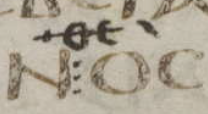
\includegraphics[width=0.3\linewidth]{img/1Tim316.png}
        \end{figure}
    \end{block}
    \end{frame}
    \begin{frame}{Variants/lectures: unintentionnels}
        \textbf{Homoioteleuton} : le scribe saute d'un mot à l'autre car ils se ressemblent. \\
        Sous-cas : Haplographie/Dittographie.\\
        \begin{block}{}
        \emph{Marc 12, 27}: \textgreek{οὐκ ἔστιν ὁ  [θεὸς?] θεὸς νεκρῶν})
        \end{block}

\end{frame}

\begin{frame}{Variants/lectures : non-intentionnels}
\textbf{Confusions d'audition}\\

\textbf{Itacism} : prononciations similaires entre différentes lettres et groupes de lettre (\textgreek{ε} $\leftrightarrow$ \textgreek{αι}, \textgreek{ο} $\leftrightarrow$  \textgreek{ω} $\leftrightarrow$  \textgreek{ῳ}, \textgreek{ο} $\leftrightarrow$ \textgreek{ο} $\leftrightarrow$ \textgreek{ο} $\leftrightarrow$ \textgreek{ο} $\leftrightarrow$ \textgreek{ο} $\leftrightarrow$ \textgreek{ο} $\leftrightarrow$)
%TODO

\begin{block}{}
   \emph{1 Co 15:54}: \textgreek{ποῦ σου, θάνατε, τὸ νῖκος ($\leftrightarrow$ τὸ νεῖκος);} (\textit{Ô mort, où est ta victoire ($\leftrightarrow$ ta controverse) ?}).
\end{block}
    
\end{frame}

\begin{frame}{Variants/lectures : intentionnels}
    \textbf{Changements liturgiques}:\\
    \begin{block}{}
    \emph{Matt 6, 13}: ajout de la doxologie \textgreek{Ὅτι σοῦ ἐστιν ἡ βασιλεία καὶ ἡ δύναμις καὶ ἡ δόξα εἰς τοῦς αἰῶνας Ἀμήν} (plusieurs onciaux et plusieurs minuscules, \textbf{Didache}) à la fin de la prière du Notre Père (plus grands codices, \textit{Sinaïticus, Vaticanus, Bezae}).
    \end{block}
\end{frame}

\begin{frame}{Variants/lectures : intentionnels}
    \textbf{Elimination d'incohérences:}\\
\end{frame}

\begin{frame}{Variants/lectures : intentionnels}
    \textbf{Harmonisations:} harmonisation entre les évangiles synoptiques.\\

    \begin{block}{}
       \emph{Luc 11, 2:4 et Matt 6, 9:13} \\
       Prière du Notre Père corrigée chez Luc pour s'aligner sur Matthieu:\\
       
        \footnotesize
       \begin{minipage}{.45\textwidth}
           \emph{Luc 6, 2:4}:\\
Père! Que ton nom soit sanctifié; que ton règne vienne. Donne-nous chaque jour notre pain quotidien; pardonne-nous nos péchés, car nous aussi nous pardonnons à quiconque nous offense; et ne nous induis pas en tentation.
       \end{minipage}
       \hfill
        \begin{minipage}{.45\textwidth}
    \emph{Matt 6, 9:13}:
Notre Père qui es aux cieux! Que ton nom soit sanctifié; que ton règne vienne; que ta volonté soit faite sur la terre comme au ciel. Donne-nous aujourd'hui notre pain quotidien; pardonne-nous nos offenses, comme nous aussi nous pardonnons à ceux qui nous ont offensés; ne nous induis pas en tentation, mais délivre-nous du malin.
       \end{minipage}
    \end{block}
\end{frame}

\begin{frame}{Variants/lectures : intentionnels}
\textbf{Harmonisations:} harmonisation entre les évangiles synoptiques.\\

\begin{block}{}
    Exemple d'harmonisations dans l'\textit{Alexandrinus}:
\end{block}

\end{frame}

\begin{frame}{Collation}
    \begin{alertblock}{}
    La \textbf{collation} est le processus de comparaison systématique des \textbf{témoins} d'un texte afin de recenser les \textbf{différentes lectures}. Elle est le point de départ de la critique textuelle.
    \end{alertblock}
    Elle est souvent représentée sous la forme d'un alignement \textbf{pour faciliter la visualisation} :
\pause

\vfill
\begin{tabular}{c|c|c|c|c|c|c}
    $\aleph$ & \textgreek{αρχη του ευαγγελιου} & \textgreek{ιυ} & \textgreek{χυ} & & & \\
    $A$  & \textgreek{αρχη του ευαγγελιου} & \textgreek{ιυ}  & \textgreek{χυ} & \textgreek{υυ} & \textgreek{του} & \textgreek{θυ}\\
    $B$ & \textgreek{αρχη του ευαγγελιου} & \textgreek{ιυ} & \textgreek{χυ} & \textgreek{υιου} & & \textgreek{θυ}\\
    $D$ & \textgreek{αρχη του ευαγγελιου} & \textgreek{ιηυ} & \textgreek{χρυ} & \textgreek{υιου} & & \textgreek{θυ}\\
    $\theta$ & \textgreek{αρχη του ευαγγελιου} & \textgreek{ιυ} & \textgreek{χυ} & & & \\
\end{tabular}
\end{frame}

\begin{frame}{Archétype}
    \begin{alertblock}{}
    L'\textbf{archétype} serait le texte d'où originerait une tradition textuelle.
    \end{alertblock}

    Il ne s'agit pas forcément de l'\emph{autographe}.
\end{frame}

\begin{frame}{Texte initial}
\textbf{L'école allemande (Münster) revoit ses termes avec l'évolution de la croyance que la critique textuelle permet de reconstruire l'archétype}:

\begin{exampleblock}{}
\emph{The Textual History of the Greek New Testament: Changing Views in Contemporary Research, SBL Press, 2011} :
    « …la définition du terme ‘texte initial’ doit être soigneusement distinguée de l’archétype de la tradition, d'une part, et du texte original de l’auteur, d'autre part. L’archétype de la tradition était un manuscrit réel, la copie par laquelle la transmission a commencé, qui a donné naissance aux manuscrits que nous possédons — ainsi qu’à beaucoup d’autres aujourd’hui perdus. Le texte original de l’auteur précède de plus d’un siècle les manuscrits que nous avons dans la plupart des cas. Le texte initial est la reconstruction hypothétique du texte tel qu’il était avant l’apparition de l’archétype de la tradition. Le texte initial est le résultat d’efforts méthodiques visant à s’approcher le plus possible du texte perdu de l’auteur en se fondant sur toutes les preuves pertinentes, sans exclure aucune trace de transmission antérieure à l’archétype. »  
\end{exampleblock}
\end{frame}

\begin{frame}{Conjecture}

\begin{alertblock}{}
    Une \textbf{conjecture} est une \textbf{lecture} proposée par l'éditeur lorsqu'aucun \textbf{témoin} ne propose une lecture satisfaisante.
\end{alertblock}

\textbf{L'édition critique contemporaine propose très peu de conjectures.}

\end{frame}

\begin{frame}{Conjectures}
    \textbf{Exemple de conjecture} (1 Jean 2,14, Jean Calvin):\\
        \begin{minipage}{.4\textwidth}
    \footnotesize
    \begin{exampleblock}{}
    \textgreek{ἔγραψα ὑμῖν, παιδία, ὅτι ἐγνώκατε τὸν πατέρα· ἔγραψα ὑμῖν, πατέρες, ὅτι ἐγνώκατε τὸν ἀπ᾽ ἀρχῆς· ἔγραψα ὑμῖν, νεανίσκοι, ὅτι ἰσχυροί ἐστε καὶ ὁ λόγος τοῦ θεοῦ ἐν ὑμῖν μένει καὶ νενικήκατε τὸν πονηρόν.}\\
    \textbf{TOB}: Je vous l'ai donc écrit, mes petits enfants, \og vous connaissez le Père \fg\.
    Je vous l'ai écrit, pères, \og vous connaissez celui qui est dès le commandement\fg. Je vous l'ai écrit, jeunes gens, \og vous êtes forts, et que la parole de Dieu demeure en vous, et que vous avez vaincu le malin\fg.\\
    \end{exampleblock}
    \end{minipage}%
    \hfill
    \begin{minipage}{.4\textwidth}
    \footnotesize
\textgreek{\emph{ἔγραψα ὑμῖν, παιδία, ὅτι ἐγνώκατε τὸν πατέρα·} ἔγραψα ὑμῖν, πατέρες, ὅτι ἐγνώκατε τὸν ἀπ᾽ ἀρχῆς· ἔγραψα ὑμῖν, νεανίσκοι, ὅτι ἰσχυροί ἐστε καὶ ὁ λόγος τοῦ θεοῦ ἐν ὑμῖν μένει καὶ νενικήκατε τὸν πονηρόν.}\\

\pause
    \textbf{Louis Segond}: Je vous ai écrit, pères, parce que vous avez connu celui qui est dès le commencement. Je vous ai écrit, jeunes gens, parce que vous êtes forts, et que la parole de Dieu demeure en vous, et que vous avez vaincu le malin.\\
    \end{minipage}
    
\end{frame}

\begin{frame}{Conjectures}
    \textbf{Exemple de conjecture} (Jean Calvin):\\
    \begin{minipage}{.4\textwidth}
    \footnotesize
    \begin{exampleblock}{}
    \textit{Has repetitiones iudico esse supervacuas. Et probabile est, cum falso putarent imperiti lectores, bis de pueris loquutum esse, temere alia duo membra supposuisse. Quanquam fieri potest, ut Ioannes ipse sententiam de adolescentibus, augendi causa, secundo inseruerit: (illic enim addit, fortes esse: quod prius non dixerat) librarii autem temere numerum implere voluerint.}
    \end{exampleblock}
    \end{minipage}%
    \hfill
    \begin{minipage}{.4\textwidth}
    \footnotesize
    \textbf{Je juge que ces répétitions sont superflues}. Et il est probable que, pensant à tort que l’auteur parlait deux fois des enfants, des lecteurs ignorants aient ajouté deux autres membres par erreur. Cependant, il est possible que Jean lui-même ait inséré la phrase sur les jeunes hommes une seconde fois pour renforcer son propos (car là, il ajoute qu'ils sont forts, ce qu'il n'avait pas dit auparavant), tandis que les copistes auraient voulu compléter le nombre de manière arbitraire.
    \end{minipage}
\end{frame}



\section{Outils et manuels}

\begin{frame}{Nestlé-Aland}
    \begin{block}{Le Nestlé-Aland}
    Le \textit{Novum Testamentum Graece} (Nestlé-Aland) est \textbf{une édition critique du texte du Nouveau Testament}, issue d'un travail collaboratif de philologues (1898-2012), qui réunit les variantes issues d'un grand nombre de témoins du Nouveau Testament.
    \end{block} 

    \textbf{Nous utiliserons seulement cette édition critique.}
\end{frame}

\begin{frame}{NTVMR}
  \begin{alertblock}{}
    Le New Testament Virtual Manuscript Room (NTVMR) est une plateforme Web financée par l'INTF de Münster qui offre un accès \textbf{aux manuscrits du Nouveau Testament}.
  \end{alertblock}
  \begin{itemize}
      \item Disponible à cette adresse : \url{https://ntvmr.uni-muenster.de};
      \item Prend un peu de temps à prendre en main, mais cela vaut le coup!
      \item Se faire un compte (gratuit) est fortement recommandé.
  \end{itemize}
\end{frame}

\begin{frame}{Manuels}
    2 livres recommandés:
\end{frame}

\begin{frame}{Questions}
    Questions ?
\end{frame}

\end{document}